\chapter{Background Theory}
\label{BackgroundTheory}
\graphicspath{{Figures/BackgroundTheory/}{Figures/Common/}}

\section{Phase-space methods}
\label{BackgroundTheory:PhaseSpaceMethods}
%Focus primarily on truncated Wigner.

\section{Absorbing boundary layers for Schrödinger-type equations}
\label{BackgroundTheory:AbsorbingBoundaryLayers}


To solve any partial differential equation numerically, it must be restricted to a finite domain with boundary conditions imposed at the edges\footnote{This requirement can be avoided when the solution's asymptotic behaviour is known \emph{a priori}, however this case will not be encountered in this thesis.}. For some systems, this poses no additional restriction over the original problem as they are explicitly defined over a finite domain and with the correct boundary conditions this constitutes the problem itself (for example electromagnetic wave propagation in a waveguide). Other systems are naturally restricted to a finite domain (for example a BEC in a trap) and will be unaffected by the imposition of the artificial boundary conditions. 

With the exception of systems defined over a finite domain, the choice of boundary conditions at the edges of the computational domain is an artificial one; while in many cases they permit physical interpretation, this interpretation does not usually correspond to the reality of the system under consideration. As an example, consider the case of a BEC freely falling under gravity. The natural domain for this problem is infinite, but to solve this system numerically it must be restricted to a finite domain. If periodic boundary conditions are used, when the BEC falls of the bottom of the computational domain, it will reappear at the top of the domain to continue falling. If the wavefunction or its derivative is set to zero on the boundary then the BEC will reflect from the bottom of the domain. Each choice of boundary condition gives different results and none correspond to the correct behaviour in which the BEC would simply fall out of the computational domain. A strategy is therefore needed to limit the effect of the choice of the boundary conditions on the solution.

A first simple strategy would be to choose the computational domain to be large enough such that no part of the atom laser beam will reach the edge of the domain over the time of interest. While effective, this strategy can be computationally expensive and is particularly demanding in the presence of gravity. Under the influence of gravity a classical particle starting from rest will travel a distance $d = \frac{1}{2}g t^2$ in time $t$. Hence the size of the computational domain must increase as $t^2$. The spatial grid separation cannot remain constant however. As the velocity of the classical particle increases as $v = gt$, the mean wavelength of the particle $\displaystyle \lambda = \frac{\hbar}{Mv}$ must then decrease as $t^{-1}$.  To resolve the spatial dynamics of the atom laser, the step size between points must then decrease as $t^{-1}$. These two effects combine to give the scaling that the total number of spatial grid points required $N_\text{pts} \propto t^3$. Choices of uniform or variable spacing for the grid will only differ by an overall constant factor in the number of points required by this strategy; such choices cannot change the overall scaling. A different strategy is needed.

In many circumstances it is the Bose-Einstein condensate and the outcoupling process that produces the atom laser that are of interest. In such situations the remainder of the atom laser that can no longer directly interact with the BEC must be prevented from doing so as a result of its unphysical interactions with the artificial boundary conditions. The solution used in the aforementioned strategy was to continue to model the atom laser, however this is not necessary. An alternative solution is to remove this part of the atom laser from the simulation in a way that has no effect on the BEC and the outcoupling process. One strategy that takes this approach is to add an \emph{absorbing boundary layer} \citep{Kosloff:1986,Neuhasuer:1989} between the domain of interest and the artificial boundary conditions. This absorbing boundary layer takes the form of a negative imaginary potential, which must be chosen to be deep enough to strongly attenuate any wave traversing it and smooth enough to make the probability of reflection negligible. \figureref{BackgroundTheory:AbsorbingBoundarySchematic} illustrates this strategy. Through the use of an appropriate absorbing boundary layer, the computational domain used to solve the system need not change and the scaling problem discussed previously will not occur.

\begin{figure}
    \centering
    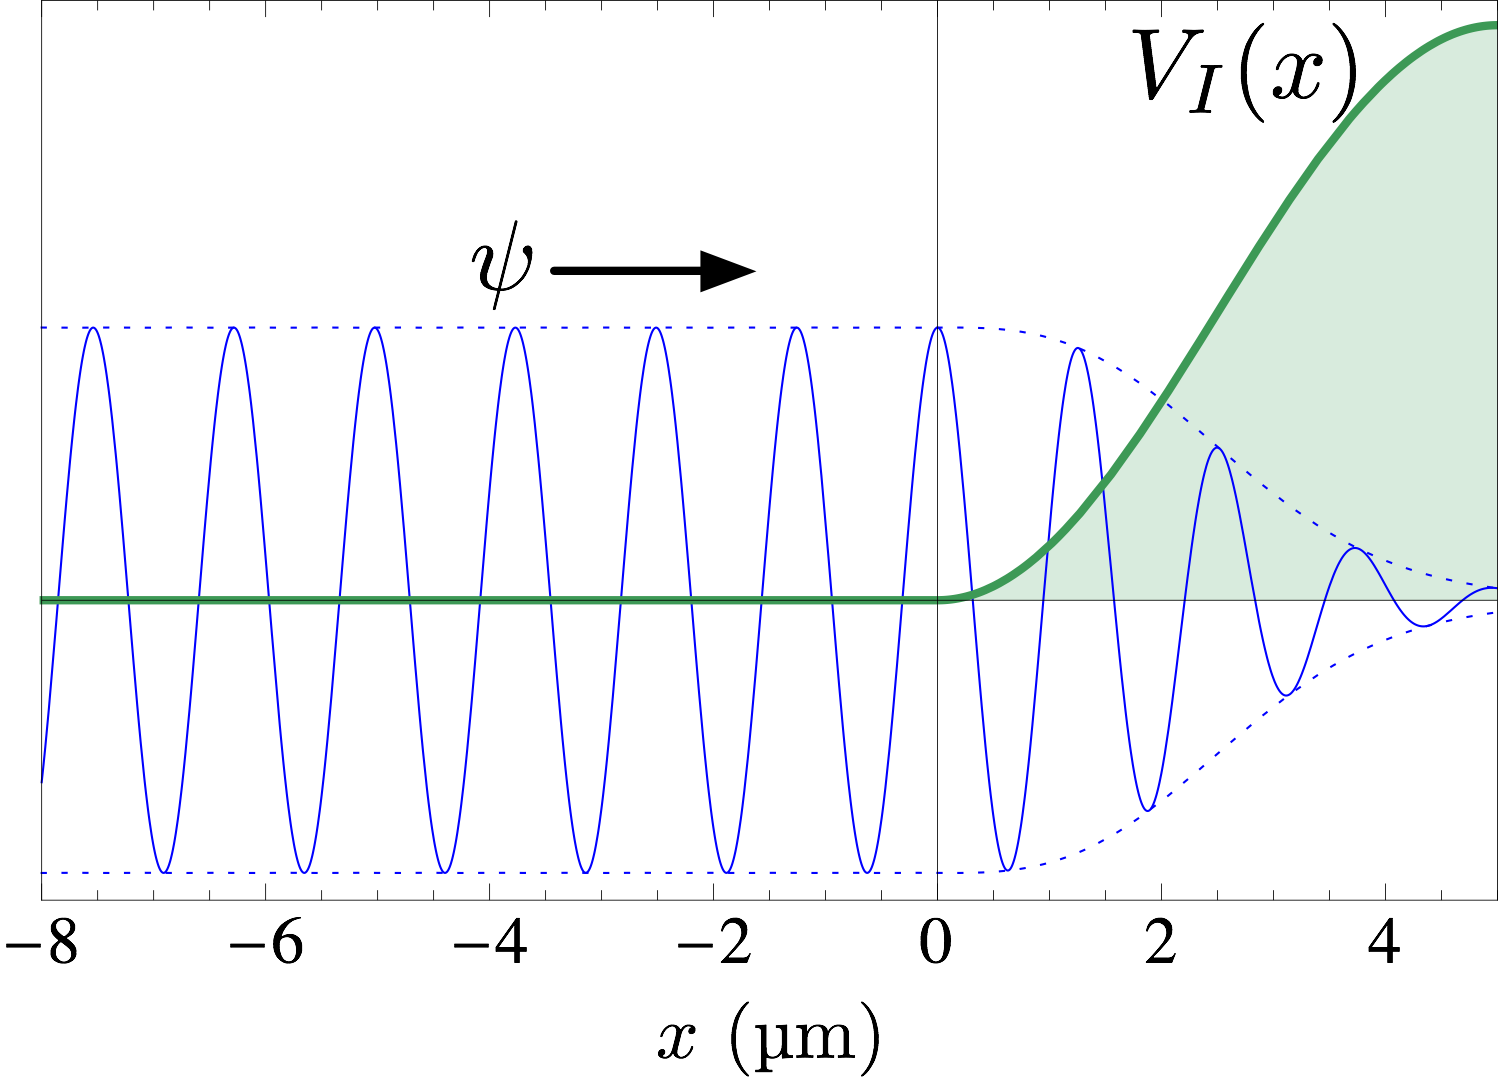
\includegraphics[width=8cm]{AbsorbingBoundarySchematic}
    \caption{
        \label{BackgroundTheory:AbsorbingBoundarySchematic}
        Schematic diagram illustrating the use of an absorbing boundary layer. A right-travelling wave is incident on the absorbing boundary layer which is given by the potential $V(x) = -i V_I(x)$. The wave is attenuated as it crosses the absorbing boundary layer.
    }
\end{figure}

An absorbing boundary layer of finite thickness can only be effective over a finite range of incident wavenumbers. Incident wavefunctions with large wavelengths (low wavenumbers) will be reflected from the absorbing boundary layer due to the rapid variation in the potential over a wavelength. Incident wavenumbers with very short wavelengths (high wavenumbers) will be transmitted through the absorbing boundary layer due to the finite amount of time spent in the absorbing boundary layer by any point on the phase-front.  Using this argument \citet{Neuhasuer:1989} showed that the approximate range of wavenumbers over which an absorbing boundary layer will be effective is
\begin{align}
    \label{BackgroundTheory:AbsorbingBoundaryKEffectiveRange}
    \left( \frac{M \overline{V_I}}{\hbar^2 \Delta x}\right)^{\frac{1}{3}} \ll k \ll \frac{4 M \overline{V_I} \Delta x}{\hbar^2},
\end{align}
where $\overline{V_I}$ is a representative value of $V_I(x)$. The maximum and minimum limits for the wavenumber are respectively due to the requirements of negligible transmission and reflection. Although cast in terms of the wavenumber, \eqref{BackgroundTheory:AbsorbingBoundaryKEffectiveRange} is equivalent to (26) in \citep{Neuhasuer:1989}. While not its purpose, \sectionref{MethodsAppendix:MomentumDensityFluxExampleCalculation} demonstrates how to calculate the reflection and transmission coefficients as a function of wavenumber for arbitrary absorbing boundary conditions.

The use of absorbing boundary layers must be slightly modified for use in phase-space methods such as those discussed in \sectionref{BackgroundTheory:PhaseSpaceMethods}. In these cases simply adding an absorbing boundary layer to the potential would lead to unphysical results as the absorbing potential would not discriminate between real particles in a mode and the virtual particles which represent the fundamental vacuum fluctuations inherent in the field. An appropriate way of handling this problem is to add a position-dependent loss term to the master equation of the form
\begin{align}
    \label{BackgroundTheory:PhaseSpaceAbsorbingBoundaryLayer}
    \frac{d \hat{\rho}}{dt} &= \int d \bm{x}\, \frac{2}{\hbar}V_I(\bm{x})\mathcal{D}[\hat{\Psi}(\bm{x})]\hat{\rho},
\end{align}
where $\mathcal{D}$ is the usual decoherence superoperator. This master equation term leads to the same imaginary potential term in the equations of motion for the field operator with an additional noise term for Truncated Wigner and the Q function methods that restores the vacuum fluctuations that would otherwise be lost.

\parasep

In most of this thesis it is only the immediate vicinity of the BEC that is under consideration and absorbing boundary layers are used to restrict the computational domain to this region. One notable exception is \chapterref{TransverseProfile} in which the transverse profile of the atom laser a large distance from the BEC is considered. In this case a different strategy must be used to avoid the $N_\text{pts} \propto t^3$ scaling discussed above. Such a strategy is discussed in \sectionref{TransverseProfile:DropGP}.

\section{Spontaneous symmetry-breaking and all that}
\label{BackgroundTheory:SymmetryBreaking}

Quantum-mechanics is \emph{linear}. If my system is in the state $\displaystyle \hat{\rho} = \sum_i P_i \ketbra{\Psi_i}{\Psi_i}$, then I can simply consider the evolution of each of the $\displaystyle \rho_i = \ketbra{\Psi_i}{\Psi_i}$ \emph{individually} and then construct the weighted average for any expectation value that I'm interested in $\mean{\hat{O}} = \sum_i P_i \bra{\Psi_i}\hat{O}\ket{\Psi_i}$. Hence, the problem of `there is no mean field' is meaningless, as we can never measure the quantity $\mean{\hat{\Psi}}$, it is only ever number-conserving operators that are physically meaningful for atoms. Because of all this, the state $\hat{\rho} = \ketbra{\Psi}{\Psi}$ where $\ket{\Psi}$ is a coherent state is physically \emph{indistinguishable} from the state $\displaystyle \hat{\rho} = \frac{1}{2\pi}\int d\phi\, \ketbra{\Psi e^{i\phi}}{\Psi e^{i\phi}}$. Hence I can make my damned mean-field approximation if I want to. And I won't hear any complaints that it is `unphysical'. Some useful papers \citep{Leggett:1991fj,Molmer:1997fr}

\section{Truncated Wigner}
\label{BackgroundTheory:TruncatedWigner}
\section{Rubidium}
\label{BackgroundTheory:Rubidium}
\section{Metastable Helium}
\label{BackgroundTheory:Helium}

\begin{table}
    \centering
    \begin{tabular}{cc}
    \toprule
    Parameter & Value\\
    \midrule
    Quasimolecule $S=0$ scattering length & $a_{S=0}=\unit[9.46]{nm}$\\
    Quasimolecule $S=2$ scattering length & $a_{S=2}=\unit[7.51]{nm}$\\
    Penning ionisation rate & $K^\text{(unpol)}_{^4\text{He}} = \unit[7.7\times 10^{-17}]{m\textsuperscript{3}}$\\
    \bottomrule
    \end{tabular}
    \caption{\label{BackgroundTheory:He*Parameters} Relevant parameters of metastable Helium.}
\end{table}

\subsection{Penning ionisation}
\label{BackgroundTheory:PenningIonisation}

The primary attraction of creating Bose-Einstein condensates of metastable helium atoms is that their large internal energy ($\unit[20]{eV}$) enables single-atom detection with high spatial (\micro m) and temporal resolution (ns). However, this large internal energy can be released when two metastable helium atoms collide resulting in Penning ionisation (PI),
\begin{align}
    \label{BackgroundTheory:PenningIonisation}
    \text{He}^* + \text{He}^* & \rightarrow \left\{
        \begin{matrix}
            \text{He}^+ + \text{He} + e^-\\
            \text{He}_2^+ + e^-
        \end{matrix}\right.
\end{align}
While this process dominates for unpolarised cold samples such as magneto-optical traps \citep{Bardou:1992}, it does not prohibit the formation of Bose-Einstein condensates as the process is suppressed by five orders of magnitude \citep{Shlyapnikov:1994} in polarised samples.  This suppression is due to conservation of angular momentum. While the reactants each have a total angular momentum $s=1$, giving their combined total angular momentum as either $S=0$ or $S=2$ (assuming $s$-wave collisions), the products each have total angular momentum $s=\frac{1}{2}$ (in the case of $\text{He}^+$, $e^-$ and $\text{He}_2^+$) or $s=0$ (for $\text{He}$), giving the total angular momentum of the products as either $S=0$ or $S=1$. Hence spin polarised states having $S=2$, $m_S=\pm2$ cannot directly undergo the process \eqref{BackgroundTheory:PenningIonisation}.

In general as $S$ is conserved, any of the $S=2$ quasimolecule states will be prevented from directly undergoing Penning ionisation. As collisions with nonzero relative angular momentum can be neglected at BEC temperatures \citep{Venturi:2000,Stas:2006kx} (due to the atoms having insufficient energy to penetrate the centrifugal barrier), it is only the $S=0$ quasimolecule state that undergoes Penning ionisation.

As derived in \sectionref{PenningIonisationAppendix:MasterEquation} the master equation term describing Penning ionisation is
\begin{align}
    \left.\frac{d \hat{\rho}}{dt}\right|_\text{PI} &= \frac{9}{2} K^\text{(unpol)}_{^4\text{He}} \int d \bm{x}\, \mathcal{D}\left[ \hat{\Xi}_{S=0, m_S=0}\right] \hat{\rho},
\end{align}
where $K^\text{(unpol)}_{^4\text{He}} = \unit[7.7\times 10^{-17}]{m\textsuperscript{3}s\textsuperscript{-1}}$ is the rate constant for the production of ions due to Penning ionisation in an unpolarised thermal sample at $\unit[1]{\micro K}$ \citep{Stas:2006kx}, and the $S=0$ quasimolecule state that undergoes Penning ionisation is given by
\begin{align}
    \hat{\Xi}_{S=0, m_S=0} &= \frac{1}{\sqrt{3}} \left( 2 \hat{\Psi}_1 \hat{\Psi}_{-1} - \hat{\Psi}_0 \hat{\Psi}_0\right).
\end{align}

